\section{Computation Graph and Data-race Detection}
\label{sec:semantics}
A Computation Graph for a task parallel program is a directed acyclic
graph representing the concurrent structure of the program execution
\cite{dennis2012determinacy}.  It is modified here to track memory
locations accessed by tasks.

\begin{definition}
A computation graph is a directed acyclic graph (DAG), $\cg = \tuple{\nodes, \edges, \rv, \wv}$, where $\nodes$ is a finite
set of nodes, $\edges \subseteq \nodes \times \nodes$ is a set of
directed edges, $\rv : (\nodes \mapsto \powerset{\glbls})$ maps $\nodes$ to
the unique identifiers for the shared locations read by the tasks,
$\wv : (\nodes \mapsto \powerset{\glbls})$ maps $\nodes$ to the unique
identifiers for the shared locations written by the tasks, and $\glbls$
is the set of the unique identifiers for the shared locations.
\end{definition}

\algoref{algo:drd} is an algorithm to analyze a computation graph for data-race with
\[
\mathit{conflict}(n_i,n_j) = 
\begin{array}{l}
  \rv(n_i) \cap \wv(n_j) \neq \emptyset\ \vee \\
  \rv(n_j) \cap \wv(n_i) \neq \emptyset\  \vee \\
  \wv(n_i) \cap \wv(n_j) \neq \emptyset\  \\
\end{array}
\]
The notation $n_i \nprec n_j$ means that $n_i$ does not precede $n_j$
in the graph. The complexity of the algorithm is
$|\glbls|*O(|\nodes|^2)$ because computing the transitive closure for
\lineref{loc:path} is $O(|\nodes|*|\edges|)$ and the \textit{conflict}
function is constant.  The algorithm is purposely naive and can be
improved if needed \cite{mellor1991fly,raman2012scalable}.  That said,
problem instances are assumed to be small enough for model checking
which dominates running time since it is limited by the number of
computation graphs that must be enumerated rather than the size of
those graphs.

\begin{algorithm}[t]
  \caption{Data Race detection in a computation graph.} \label{algo:drd}
\begin{algorithmic}[1]
\Function{data\_race}{$\tuple{\nodes, \edges, \rv, \wv}$}
\For {\textbf{each} $n_i,n_j \in \nodes$}
\If {$(n_i \nprec n_j) \wedge (n_j \nprec n_i)$}  \label{loc:path} \label{loc:forall}
   \If {\textit{conflict}$(n_i,n_j,\rv,\wv)$}
      \State {report data-race} \label{loc:datarace}
      \EndIf
\EndIf
 \EndFor
\EndFunction  
\end{algorithmic}
\end{algorithm}


\begin{figure}
  \centering
        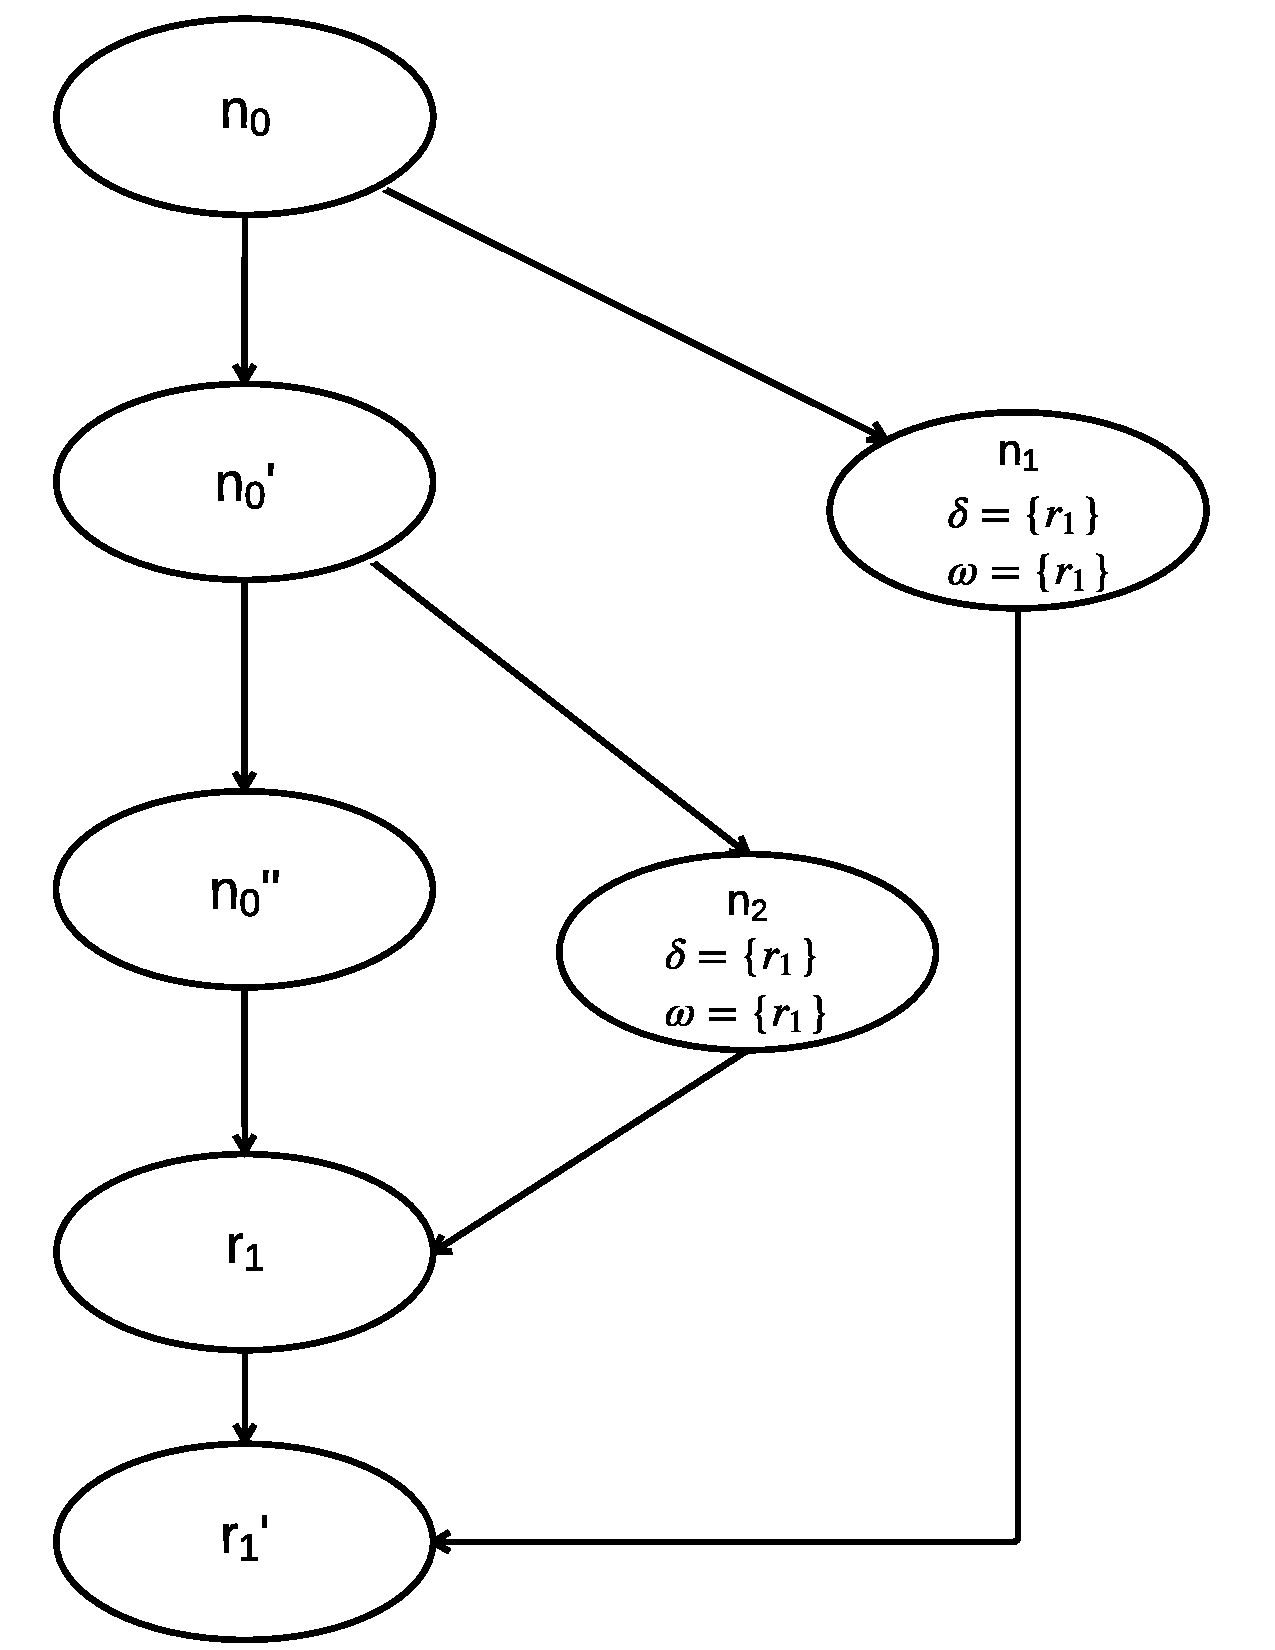
\includegraphics[width=0.3\textwidth]{../figs/Fig3-1.pdf}
    \caption{Computation Graph Example.}
    \label{fig:cg}
    \vspace{-1em}
\end{figure}

\section{Task Parallel Programs} \label{sec:cg}
This section formally defines how to build a computation graph from an
execution trace of a task parallel program.  The programming model is
derived from Bouajjani and Emmi for isolated parallel tasks
\cite{bouajjani}; this variant removes the isolation between tasks
with the introduction of shared memory. It additionally restricts task
passing to only allow tasks to be passed when a child completes, and
those tasks are only passed to the parent.

\subsection{Syntax}
The surface syntax for the language is given in \figref{fig:syntax}.
A program \textbf{P} is a sequence of procedures.  The procedure name
$p$ is taken from a finite set of names \texttt{Proc}.  Each procedure
has a single $L$-type parameter \texttt{l} taken from a finite set of
parameter names \texttt{Vars}; restricting to a single-parameter simplifies the presentation and has no bearing on results.  The
semantics is abstracted over concrete values and operations, so the
possible types of \texttt{l} are not specified. Procedures may also
reference shared variables taking from a finite set of names, $\glbls$,
where $\glbls \cap \mathtt{Vars} = \emptyset$. The names include a
special reserved variable \texttt{isolate} that is only used by the
semantics for mutual exclusion.

The body of a procedure is inductively defined by \textbf{s}.  The
expression language, $e$, is also abstracted and not specified, but
assume it includes variables, references, and a finite set of values
,\texttt{Vals}, that include at least Boolean values.  The set of all
expressions is given by \texttt{Exprs}.

\begin{figure}
  \begin{center}
\[
  \begin{array}{rcl}
\textbf{P} &::=& (\textbf{proc}~p~(\textbf{var}\ \texttt{l} : L)~s)* \\
\textbf{s} &::=& s;~s \alt \texttt{l} := e \alt \textbf{skip} \alt [ \textbf{if}~e~\textbf{then}~s~\textbf{else}~s ] \\
&\alt& [ \textbf{while}~e~\textbf{do}~s ] \alt \textbf{call}~\texttt{l}\ := p~e \alt \textbf{return}~e \\
&\alt& \post~r \leftarrow p~e~d \alt \await~r \alt \ewait~r \\
&\alt& [ \isolated~s ]
  \end{array}
\]
  \end{center}
  \caption{The surface syntax for task parallel programs.}
  %\vspace{-2em}
  \label{fig:syntax}
\end{figure}

The \post-statement, \await-statement, \ewait-statement, and
\isolated-statement relate to concurrency; the rest of the statements
have their usual sequential meaning.  The \post-statement adds a task
into a region $r$, taken from a finite set of region identifiers,
\texttt{Regs}, by indicating the procedure $p$ for the task with an
expression for the local variable value $e$, and a return value
handler $d$ to run in the context of the parent task.  Let
\texttt{Stmts} be the set of all statements and let $\texttt{Rets}
\subseteq (\texttt{Vals} \rightarrow \texttt{Stmts})$ be the set of
return value handlers.

The \await\ and \ewait\ statements synchronize a task with the
sub-ordinate tasks in the indicated region.  Intuitively, when a task
calls \await\ on region $r$, it is blocked until all the tasks it owns
in $r$ finish execution.  Similarly, when a task issues an
\ewait\ with region $r$, it is blocked until one task it owns in $r$
completes.  A task is termed \emph{completed} when its statement is a
\textbf{return}-statement.

The \isolated-statement provides mutual exclusion relative to other
\isolated-statements.  If $s$ is isolated, then it runs mutually
exclusive to any other statements $s^\prime$ that are also isolated;
however, $s$ does not run mutually exclusive to other non-isolated
statements that may be concurrent with $s$.

In addition to the restrictions created by the syntax, we assume that
all programs adhere to the following additional restriction:
procedures with side-effecting return value handlers must be the only
members of their respective regions. This restriction is common to
task-parallel languages.

\subsection{Tree-based Semantics}

The semantics of task parallel programs is defined over trees of
procedure frames to represent the parallelism in the language rather
than stacks which are inherently sequential.  That means that the
frame of each posted task becomes a child to the parent's frame. The
parent-child relationship is transferred appropriately when a parent
completes without synchronizing with its children.  The evolution of
the program proceeds by a task either taking a sequential step or a
concurrency related step that creates, synchronizes, or orders with
other tasks.  The semantics additional define the construction of the
computation graph that is also part of the program state.

A task $t = \tuple{\ell, s, d, n}$ is a tuple containing the value,
$\ell$, of the procedure local variable \texttt{l}, along with a
statement $s$, a return value handler $d$, and an associated node,
$n$, in the computation graph for this task.

A \emph{tree configuration}, $c = \tuple{t,m}$, is an inductively
defined tree with task-labeled vertexes, $t$, and region labeled edges
given by the \emph{region valuation} function, $m : \texttt{Regs}
\rightarrow \texttt{Configs}$, where \texttt{Configs} is the set of
tree configurations.  For a given vertex $c = \tuple{t,m}$, $m(r)$
returns the collection of sub-trees connected to the $t$-labeled root
by $r$-labeled edges. In this context, $m$ is local to the current
task frame. Let $m_o$ be the initial region valuation such that
$\forall r \in \mathtt{Regs}, m_o(r) = \emptyset$.

Contexts are used to simplify the rules for the semantics. A
\emph{configuration context}, $C$, isolates individual task
transitions in the tree (e.g., $C[\tuple{t,m}] \rightarrow
C[\tuple{t^\prime,m}]$ denotes a transition on a
task). Similarly, a \emph{statement context}, $S$, indicates the next
statement to be executed.  A \emph{task statement context}, $T =
\tuple{\ell, S, d, n}$ is a task with a statement context in place of
a statement, and likewise $T[s]$ indicates that $s$ is the next
statement to be executed in the task. Like configuration contexts,
task statement contexts isolate the statement to be executed (e.g.,
$C[\tuple{T[s_1],m}] \rightarrow C[\tuple{T[s_2],m}]$ denotes a transition that modifies the statement in some way).

The \emph{state} of a task parallel program is $\tuple{\cg, \sigma,
  \tuple{t,m}}$ where $\cg$ is a computation graph, $\sigma:
\glbls \rightarrow \mathtt{Vals}$ is a partial function mapping global
variable names in $\glbls$, and $\tuple{t,m}$ is the configuration context for the root of the tree. 

Let $\llbracket \cdot \rrbracket_e$ be an partial evaluation function
for expressions without any variables. For convenience in the
semantics:
\begin{eqnarray*}
  e(t, \sigma) &=& e(\tuple{\ell, s, d, n}, \sigma) \\
  &=& e(\ell, \sigma) \\
  &=& \llbracket e[\ell / \texttt{l}, \sigma(\mathtt{g}_0) / \mathtt{g}_0, \sigma(\mathtt{g}_1) / \mathtt{g_1}, \ldots]  \rrbracket_e
  \end{eqnarray*}
If $e[\ell / \texttt{l}, \sigma(\mathtt{g}_0) / \mathtt{g}_0,
  \sigma(\mathtt{g}_1) / \mathtt{g_1}, \ldots]$ has any free variables
or other errors, then by definition, \\ $\llbracket e[\ell /
  \texttt{l}, \sigma(\mathtt{g}_0) / \mathtt{g}_0,
  \sigma(\mathtt{g}_1) / \mathtt{g_1}, \ldots] \rrbracket_e$ has no
meaning and is undefined. The function is naturally extended to used
contexts as indicated by $e(T)$.  Finally, let the set of shared
variables that appear in $e$ be denoted by $\eta(e,\sigma)$.

As indicated previously, a task $t$ is completed when its next to be
executed statement $s$ is \textbf{return} $e$. Its return-value
handler statement is $\mathrm{rvh}(t) = d(e(T))$ given the task's
context.  By definition, $\mathrm{rvh}(t)$ undefined when $t$ is not
completed or $e(T)$ is undefined.

Finally, the notation, $\rho^\prime = \rho[n \bowtie \eta(e,\sigma)]$
with $\bowtie \in \{\mapstou,\mapsto\}$, indicates the $\rho^\prime$
is just like $\rho$ only if $\bowtie = \mapstou$, then $\rho^\prime(n)
= \rho(n) \cup \eta(e,\sigma)$, and if $\bowtie = \mapsto$, then
$\rho^\prime(n) = \eta(e,\sigma)$. The notation, $m_1^\prime = m
\setminus (r \mapsto \tuple{t_2,m_2})$ means that $m_1^\prime$ is just
like $m$ only $m(r)$ does not include $\tuple{t_2,m_2}$.

The semantics produce a computation graph as a by-product of reducing
the program. Two additional data are associated with the computation
graph and are used by the semantics in the construction: $\last$ is a
special node used to assert the observed order of \isolated-statements
and $\regnodemap : \mathtt{Regs} \mapsto \powerset{\nodes}$ is a function used
to join tasks in a region at synchronization.  In general, a function
notation is adopted to access members of tuples. For example, the
members of the $cg = \tuple{\nodes,\edges, \rv,\wv,\last,\regnodemap}$ are accessed as $\nodes(\cg)$, $\edges(\cg)$,
$\rv(\cg)$, etc.


\begin{figure}
  \begin{center}
    \mprset{flushleft}
    \begin{mathpar}
      \inferrule[Post]
                {
                  n_0^\prime = \mathrm{fresh}() \\
                  n_1 = \mathrm{fresh}() \\
                  \nodes(\cg^\prime) = \nodes(\cg) \cup \{n_0^\prime, n_1\} \\
                  \edges(\cg^\prime) = \edges(\cg) \cup \{\tuple{n_0, n_0^\prime}, \tuple{n_0, n_1}\}\\
                  \rv(\cg^\prime) = \rv(\cg)[n_0 \mapstou \eta(e,\sigma)]\\\\
                  \ell = e(\ell^\prime,\sigma) \\
                  m^\prime = m[r \mapstou \tuple{\tuple{\ell, s_p, d,n_1},m_o}]
                }
                {
                  \tuple{\cg,\sigma,C[\tuple{\ell^\prime,
                        S[\post~r \leftarrow p~e~d],d^\prime, n_0}, m]} \rightarrow \\
                  \tuple{\cg^\prime,\sigma,C[\tuple{\ell^\prime,
                        S[\textbf{skip}],d^\prime, n_0^\prime}, m^\prime]}
                }
      \and
      \inferrule[Await]
                {
                  \regnodemap(\cg^\prime) = \regnodemap(\cg)[r \mapstou \node(t_2)] \\
                  \rv(\cg^\prime) = \rv(\cg)[\node(t_2) \mapstou \eta(e,\sigma)]\\
                  m_1 = m \setminus (r \mapsto \tuple{t_2,m_2}) \\
                  (m_1 \cup m_2)(r) \neq \emptyset \\
                  s(t_2) = \mathbf{return}\ e \\
                  s = d(e(t_2, \sigma))
                }
                {
                  \tuple{\cg,\sigma,C[\tuple{\ell,
                        S[\await~r],d, \node}, m]} \rightarrow \\
                  \tuple{\cg^\prime, \sigma, C[\tuple{\ell,
                        S[s;~\await~r],d, \node}, m_1 \cup m_2]}
                }
      \and
      \inferrule[Await-done]
                {
                  n^\prime = \mathrm{fresh}() \\
                  \nodes(\cg^\prime) = \nodes(\cg) \cup \{\node^\prime\} \\
                  \edges(\cg^\prime) = \edges(\cg) \cup \{\tuple{\node, \node^\prime},\tuple{\node(t_2), \node^\prime}\} \cup
                  \{\tuple{\node_i,\node^\prime} \mid \node_i \in \regnodemap(\cg)(r)\} \\
                  \regnodemap(\cg^\prime) = \regnodemap(\cg)[r \mapsto \emptyset] \\
                  \rv(\cg^\prime) = \rv(\cg)[\node(t_2) \mapstou \eta(e,\sigma)]\\
                  m_1 = m \setminus (r \mapsto \tuple{t_2,m_2}) \\
                  (m_1 \cup m_2)(r) =
                  \emptyset \\
                  s(t_2) = \mathbf{return}\ e \\
                  s = d(e(t_2, \sigma))
                }
                {
                  \tuple{\cg,\sigma,C[\tuple{\ell,
                        S[\await~r],d, \node}, m]} \rightarrow \\
                  \tuple{\cg^\prime, \sigma, C[\tuple{\ell,
                        S[s],d, \node^\prime}, m_1 \cup m_2]}
                }
      \and
      \inferrule[Isolated]
                {
                  n^\prime = \mathrm{fresh}() \\
                  \nodes(\cg^\prime) = \nodes(\cg) \cup \{n^\prime\} \\
                  \edges(\cg^\prime) = \edges(\cg) \cup \{\tuple{n, n^\prime},  \tuple{\last(\cg),n^\prime}\}\\
   				  \sigma(\mathtt{isolate}) = \falsev \\
                  \sigma^\prime = \sigma[\mathtt{isolate} \mapsto \truev]
                }
                {
                  \tuple{\cg,\sigma,C[\tuple{\ell^\prime,S[\isolated~s],d^\prime, n, 0}, m]} \rightarrow \\
                  \tuple{\cg^\prime, \sigma^\prime, C[\tuple{\ell^\prime,
				        S[s; \textbf{isolated-end}],d^\prime, n^\prime, 1}, m]}
                }
      \and
      \inferrule[Isolated-done]
                {
                  n^\prime = \mathrm{fresh()}\\
                  \last(\cg^\prime) = n \\
                  \nodes(\cg^\prime) = \nodes(\cg) \cup \{n^\prime\} \\
                  \edges(\cg^\prime) = \edges(\cg) \cup \{\tuple{n, n^\prime}\} \\
                  \sigma(\mathtt{isolate}) = \truev \\
                  \sigma^\prime = \sigma[\mathtt{isolate} \mapsto \falsev]
                }
                {
                  \tuple{\cg, \sigma, C[\tuple{\ell^\prime,S[\textbf{isolated-end}],d^\prime, n, 1}, m]} \rightarrow \\
                  \tuple{\cg^\prime, \sigma^\prime, C[\tuple{\ell^\prime,
				   S[\textbf{skip}],d^\prime, n^\prime,0}, m]}
                }
                
\end{mathpar}
  \end{center}
  \caption{The transition rules for the inter-procedural statements, task creation, and task synchronization.}
%    \vspace{-2em}
  \label{fig:inter}
    \label{fig:semantics}
\end{figure}

The semantics is given as a set of transition rules relating states.
\figref{fig:inter} contains a subset of the rules pertinent to the
proof of correctness in the next section. The omitted rules for
intra-procedural statements have their usual definition; additionally, the
inter-procedural statement, $\textbf{call}~\texttt{l}\ := p~e$, is
syntactic sugar for
\[
\post~r_\mathit{call}\leftarrow p~e~\lamdefe{v}{\texttt{l} := v};~
\ewait~r_\mathit{call},
\]
where $r_{call}$ is exclusive to the caller containing no other tasks. The semantics create a computation graph as a byproduct of reducing the program. The computation graph observes rather than determines the execution of the program. 

The \textsc{Post} rule creates a new child task. The rule adds two
fresh nodes $n_0^\prime$ and $n_1$ to the computation graph: node
$n_0^\prime$ represents the statements following \post\ and $n_1$
represents the statements to be executed by the new task. The rule
orders both after the current node for the parent, $n_0$, in the
computation graph.  The read set $\rho$ of node $n_0$ is updated to
include any global variables referenced in the expression,
$\eta\left(e\right)$, for the local parameter value in the new
task. The region mapping $m$ of the parent task is updated to include
the new task with its empty initial region mapping.


The \textsc{Await} rule blocks the execution of the currently
executing task until a task in the indicated region completes.  A new
node to join the two tasks is not created in the computation graph,
nor are the two tasks ordered in the sense of join because the choice
of task $t_2$ in the region is non-deterministic; as such, the
computation graph allows tasks in the region to join in any order
contrary to the observed reduction by the rule. The rule saves the
current node in the graph for $t_2$, $\node(t_2)$, to join later once
the region is empty, and it updates the read set for $t_2$ on the
expression in the \textbf{return}-statement. The rest of the rule
separates out the task from the region, makes sure the region is not
yet empty, and gets the statement for the return value handler. The
new state adds an \textbf{await}-statement after the return value
handler statement since the region is not yet empty, and the region
valuation function in the new state includes any tasks owned by
$t_2$.\footnote{The region valuation $m_2$ may actually include tasks
  posted into $r$ because configurations are local rather than
  global. This locality means that two tasks may post into the same
  region, but neither tasks knows about the tasks posted by the other
  into that region.}


The \textsc{Await-Done} activates when the last task in the region is
joined. It differs from the \textsc{Await} rule in that it
orders all tasks that have joined in the region to happen-before the
new node for the parent in the computation graph, and it does not
insert another \textbf{await}-statement in the new state.

The \textsc{Ewait} and \textsc{Ewait-Done} rules, not shown in the
figure, follow \textsc{Await} and \textsc{Await-Done} respectively
only without the recursive statement when the region is not empty
since it only needs to wait on a single task to complete. The rules
delay the ordering of tasks joined in the region to when the region
becomes empty (i.e., the last task joins) just as done for
\textbf{await}-statements.

If no other isolated statements are running, then the
\textsc{Isolated} rule updates the \texttt{isolated} shared variable
and inserts after the isolated statement $\mathit{s}$ the new
\textbf{isolated-end} keyword. The computation graph gets a new node
to track accesses in the isolated statement with an appropriate edge
from the previous node. A sequencing edge from $\last$ is also added
so the previous isolated statement happens before this new isolated
statement. As a note, $\last$ is initialized to the initial node when
execution starts.

The \textsc{Isolated-End} rule creates a new node in the computation
graph to denote the end of isolation, updates the \texttt{isolated}
shared variable, and it updates $\last$ to properly sequence any
future isolation. \textbf{isolated}-statements are totally ordered in
the computation graph.

The initial task for a program is $t_o = \tuple{\ell, s_o,
  \lamdefe{v}{\mathtt{skip}}, n}$ where $\ell$ is the initial value of
the parameter for the top level procedure $p_o$, $s_o = \post r_0
\leftarrow p_0~\ell~\lamdefe{v}{\mathtt{skip}}; \await~r_0$;
$\await~r_1; \ldots$, and $n$ is a fresh node for the computation
graph (i.e., $n = \mathrm{fresh}()$). The initial state of a program
is given as $\tuple{\cg_o, \sigma_o, \tuple{t_o,m_o}}$ where $\cg_o$
is an initial graph such that $N = \{n\}$, $E = \emptyset$, $\rho(n) =
\emptyset$, and $\omega(n) = \emptyset$; $\sigma_o$ maps all global
variables to an initial default value; and $\forall r \in
\texttt{Regs}, m(r) = \emptyset$.

